\documentclass[11pt]{article}

\usepackage{natbib}
\usepackage{setspace}
\usepackage[left=2.5cm,top=2.8cm,right=2.5cm,bottom=2.8cm]{geometry}
\usepackage{graphicx}
\usepackage{amsmath}
\usepackage{theorem}
\usepackage{version}
\usepackage{multirow}
\usepackage{listings}
\usepackage{hyperref}
\usepackage{amssymb}
\usepackage{tikz}
\usepackage{algorithm}
\usepackage{algorithmic}
\usetikzlibrary{arrows,arrows.meta,decorations,decorations.pathreplacing,calc,matrix}

\definecolor{Red}{rgb}{1,0,0}
\definecolor{Blue}{rgb}{0,0,1}
\definecolor{Green}{rgb}{0,1,0}
\definecolor{magenta}{rgb}{1,0,.6}
\definecolor{lightblue}{rgb}{0,.5,1}
\definecolor{lightpurple}{rgb}{.6,.4,1}
\definecolor{gold}{rgb}{.6,.5,0}
\definecolor{orange}{rgb}{1,0.4,0}
\definecolor{hotpink}{rgb}{1,0,0.5}
\definecolor{newcolor2}{rgb}{.5,.3,.5}
\definecolor{newcolor}{rgb}{0,.3,1}
\definecolor{newcolor3}{rgb}{1,0,.35}
\definecolor{darkgreen1}{rgb}{0, .35, 0}
\definecolor{darkgreen}{rgb}{0, .6, 0}
\definecolor{darkred}{rgb}{.75,0,0}
\definecolor{lightgrey}{rgb}{.7,.7,.7}

\definecolor{clemson-orange}{RGB}{234,106,32}
\definecolor{chicago-maroon}{RGB}{128,0,0}
\definecolor{northwestern-purple}{RGB}{82,0,99}
\definecolor{cornell-red}{RGB}{179,27,27}
\definecolor{sauder-green}{RGB}{171,180,0}
%\definecolor{gray}{RGB}{192,192,192}
\definecolor{lawngreen}{RGB}{0,250,154}

\setcounter{MaxMatrixCols}{10}

\onehalfspacing
\newtheorem{theorem}{Theorem}
\newtheorem{acknowledgement}{Acknowledgement}
\newtheorem{algorithm}{Algorithm}
\newtheorem{assumption}{Assumption}
\newtheorem{axiom}{Axiom}
\newtheorem{case}{Case}
\newtheorem{claim}{Claim}
\newtheorem{conclusion}{Conclusion}
\newtheorem{condition}{Condition}
\newtheorem{conjecture}{Conjecture}
\newtheorem{corollary}{Corollary}
\newtheorem{criterion}{Criterion}
\newtheorem{definition}{Definition}
\newtheorem{example}{Example}
\newtheorem{exercise}{Exercise}
\newtheorem{lemma}{Lemma}
\newtheorem{notation}{Notation}
\newtheorem{problem}{Problem}
\newtheorem{proposition}{Proposition}
{\theorembodyfont{\normalfont}
\newtheorem{remark}{Remark}
}
\newtheorem{summary}{Summary}
\newenvironment{proof}[1][Proof]{\textbf{#1.} }{\hfill \rule{0.5em}{0.5em} \bigskip}
\newenvironment{soln}[1][Soln]{\textbf{#1:} }{\hfill \rule{0.5em}{0.5em}}
\renewcommand{\cite}{\citeasnoun}
\renewcommand{\theenumii}{(\alph{enumii})}
\renewcommand{\labelenumii}{\theenumii}
\renewcommand{\theenumiii}{\roman{enumiii}}
\renewcommand{\labelenumiii}{\theenumiii.}

\usepackage[nameinlink]{cleveref}
\crefname{assumption}{Assumption}{Assumptions}
\crefname{lemma}{Lemma}{Lemmas}
\crefname{theorem}{Theorem}{Theorems}
\crefname{corollary}{Corollary}{Corollaries}
\crefname{proposition}{Proposition}{Propositions}
\crefname{claim}{Claim}{Claims}
\crefname{procedure}{Procedure}{Procedures}
\crefname{algorithm}{Algorithm}{Algorithms}
\crefname{figure}{Figure}{Figures}
\crefname{remark}{Remark}{Remarks}
\crefname{section}{Section}{Sections}
\crefname{procedure}{Procedure}{Procedures}
\crefname{example}{Example}{Examples}
\crefname{definition}{Definition}{Definitions}
\crefname{table}{Table}{Tables}
\crefname{align}{}{}
\crefname{enumi}{}{}
\crefname{conjecture}{Conjecture}{Conjectures}
\crefname{step}{Step}{Steps}
\crefname{appendix}{Appendix}{Appendices}
\crefname{footnote}{Footnote}{Footnotes}

\begin{document}


\begin{center}
    \textbf{CS 326 - Analysis of Algorithms - HW 2}\\
\end{center}


\begin{flushleft}
    \textit{Prof. M. Grigni\hfill09/22/2022 \hfill Hridansh Saraogi} \\
    \vspace{0.15cm}
    \small {Help taken from: Prof. Grigni, and Zhenke Liu}\\
    \small {Collaborators: Rhea Ramchandran}
\end{flushleft}


\begin{enumerate}

\item Problem 1. Shifted Recurrence. \\
For positive integers n, define T(n) using this recurrence:
\begin{equation}
T(n) = 
\left\{
    \begin{array}{lr}
        n & \text{for }  1 \leq n \leq 10,\\
        2*(T( \lfloor n/2 \rfloor + 5)+n, & \text{for } n\geq 11.
    \end{array}
\right\}
\end{equation}
Our goal is to show $T(n) = O(n*lg n)$, without using the Master Theorem. (This resembles the mergesort recurrence, except for the "+5" shifting term. In this problem we show that we get the same asymptotic upper bound.)

    \begin{enumerate}
        \item Argue that $T(n)$ is non-decreasing. That is, $T(n) \leq T(n+1)$ for all $n \geq 1$. Use induction.
        
        \begin{enumerate}
            \item Let P(n) be the statement: $T(n) \leq T(n+1)$
            \item Base Case: Check that $T(n) \leq T(n+1)$ is true for $1 \leq n \leq 10$
            \begin{enumerate}
                \item $n = 1: T(1) = 1; T(n+1) = T(1+1) = T(2) = 2$\\
                Since $2 >1$, P(n) holds true
                \item n = 3: T(3) = 3; T(n+1) = T(3+1) = T(4) = 4\\
                Since $4 > 3$, P(n) holds true
                \item n = 6: T(6) = 6; T(n+1) = T(6+1) = T(7) = 7\\
                Since $7 > 6$, P(n) holds true
                \item n = 7: T(7) = 7; T(n+1) = T(7+1) = T(8) = 8\\
                Since $8 > 7$, P(n) holds true
                \item n= 10: T(10) = 10; T(n+1) = T(10+1) = T(11) = 2*(T(11/2) + 5) + 11 \\
                = 2*(T(5) + 5) + 11
                = 2*(5+5) + 11 = 2*10 + 11\\
                = 20 + 11 = 31\\
                Since $31 > 10$, P(n) holds true. This was an edge case but P(n) still held true
            \end{enumerate}
            Given all the above cases (instead of checking for all 10 possible values of n in this piece-wise segment, we randomly selected a few), we see that $T(n) \leq T(n+1)$.
            Further, it is also important to note that the derivative of $T(n) \leq T(n+1)$ for $1 \leq n \leq 10$ is 1. This means that is is an increasing function.\\
            $\therefore$ we can conclude that the Base Case is true
            
            \item Now let us utilise the method of Strong Induction to prove that the recurrence T(n) holds true for the entire function\\
            Let us assume $T(n-1) \leq T(n)$, for $n \leq k$ and must be smaller than 12 ($k > 12$)
            \item Using the above, we will see if P(n) holds true. Based on this, we get:\\
            $\lfloor k/2 \rfloor + 5 \leq \lfloor (k+1)/2 \rfloor + 5 \leq k$
            \item By applying both sides of the inequality to the T(n) function, we get:\\
            $T(\lfloor k/2 \rfloor + 5) \geq T(\lfloor (k+1)/2 \rfloor + 5)$
            \item Since $k < k+1$, we can insert the same into the above inequality to obtain:\\
            $2*T(\lfloor k/2 \rfloor + 5) + n \hspace{1cm}\leq \hspace{1cm}$ $ 2*T(\lfloor (k+1)/2 \rfloor + 5) + k + 1$
            \item This signifies that $T(k) \leq T(k+1)$, and hence can claim that it is an increasing function.\\
            $\therefore T(n)$ is non-decreasing
            
        \end{enumerate}

        \item Find constants c and d, so that $T(2^k+10) \leq 2^k(k+c)-d$ for all integers $k \geq 10$. Use induction on k, and give explicit values for c and d.
        \begin{enumerate}
            \item Let's consider the Base Case where k = 0\\
            In this case, $T(11) \leq 2^0(0+c) - d$\\
            As calculated previously, T(11) = 31. So we get $31 \leq c-d$
            \item Let us focus on the situation where $k \geq 1$. This will help when proving the induction
            \item We will make the following assumption:\\
            $T(2^{k-1} + 10) \leq 2^{k-1} * (k-1+c)-d$
            \item The above was for k-1. Let us obtain for k. Please see below\\
            $T(2^k + 10) = 2 * T(2^{k-1} + 10) + 2^k + 10 \leq 2(2^{k-1}(k-1 + c)-d)+2^k + 10$
            \item Simplifying: 
            $2(2^{k-1}(k-1 + c)-d)+2^k + 10 =2^k(k+c)-2d+10$
            \item Using the above inequality, we comprehend that $2^k(k+c)-2d+10 \leq 2^k*(k+c)-d$ is necessary to make the following inequality hold:\\
            $T(2^k+10) \leq 2^k(k+c)-d$
            \item This gives us that d must always be greater than or equal to 10 ($d \geq 10$)
            \item Using the above requirement, and the one we found at the start of this sub-section, based on T(11): $31 \leq c-d$\\
            We can conclude that the following numbers satisfy both the above requirements:\\
            c = 41 & d = 10
        \end{enumerate}

        \item Using (a) and (b), conclude that T(n) is $O(n* lg n)$.
        \begin{enumerate}
            \item From subpart b of Q1, we obtained the following:\\
            $T(2^k + 10) \leq 2^k (k + c) - d$
            \item Now, to conclude that T(n) is $O(n* lg n)$, let us find the smallest k so that $n \leq 2^k + 10$
            \item This gives us:\\
            $2^k \geq (n-10)$\\
            $k \geq lg(n-10)$
            \item we also know: $n \geq 11$, if $n=2^k + 10 \rightarrow k \geq 0$
            \item Using subpart a of Q1, we saw that $T(n) <= T(2^k + 10)$\\
            This helps us arrive at the following:\\
            $T(n) \leq 2^k (k+c) - d \leq (n-10)(log(n-10)+41)-10$
            \item $(n-10)(log(n-10)+41)-10 \leq n*(log(n)+41)-10 \leq n*log(n) + 41n - 10$
            \item This has the complexity of O(n*log(n))
            \item Now let us use bounds to confine n-10's range. The lowest it can go is $2^{k-1}$ and the greatest it can be is $2^k$\\
            This helps us compute the value for n
            \item On the lower bound: $2^{k-1} < n-10$\\
            $k-1 < log(n-10) \rightarrow k < 1 + log(n)$
            \item Using subpart b of Q1:\\
            $T(2^{1 + log(n} + 10) \leq 2^{1+log(n)} (1+log(n)+c)-d$
            \item We need to use the following understanding to continue this further\\
            Since $\frac{2^n+10}{2^{n-1}+10}\leq 2$, we get:\\
            $T(n) \leq n*(log(n - 10) + 41) - 10 \leq n*(log(n)+41) - 10$ \\
            This understanding helps us continue $T(2^{1 + log(n} + 10) \leq 2^{1+log(n)} (1+log(n)+c)-d$
            \item $T(2*2^{log(n)}+ 10) \leq (2*2^{log(n)})(1 + log(n) + 41)-10$\\
            $T(2n + 10) \leq 2n + 2n*log(n) + 41*(2n)-10$
            \item $T(n) \leq 2n*log(n) + 2n + 82n -10$\\
            Based on complexity analysis, the first term in the above equation would be the most complex
            $\therefore T(n) = O(n*log(n))$
        \end{enumerate}
        
    \end{enumerate}
\pagebreak
\item Problem 2. Selection in Two Sorted Arrays.\\
Suppose A[1..m] and B[1..n] are two sorted arrays of numbers, and that the m+n numbers are all distinct. We are also given an integer i, $1 \leq i \leq m+n$. We want to return the $i^{th}$ smallest number, in the union of A and B. Like in Chapter 9: i=1 means we should return the minimum, i=m+n means we should return the maximum. Using pseudocode, write out a procedure solving this problem, and argue that it runs in O(lg(m+n)) time.  Your solving procedure may be recursive, and it probably works on subarrays of the original arrays, for example: solve(A,p1, r1, B, p2, r2, i).\vspace{0.1cm}

\textbf{Hints: }If m or n is zero, the problem is easy. While both arrays are nonempty, compare the median of A with the median of B. Then depending on the comparison and i, you have enough information to eliminate either half of A or half of B.\\

\textbf{Solution: }\\
Some things to keep in mind
\begin{enumerate}
    \item m + n is always greater than or equal to 1
    \item If it is =1, that means one of the arrays is of length 0\\
    In such a case, immediately, the non-0 array's $i^{th}$ element will be returned
\end{enumerate}

Some tricks/strategies to improve computational speed (inspiration from MergeSort technique)
\begin{enumerate}
    \item Look at mid-points of each array & compare to:\\
    The below situation will work because all the m+n numbers are distinct
    \begin{enumerate}
        \item Let's look at sum of the indices of the middle elements of each array\\
        If it is greater than i, let's compare index of a particular array to i
        \begin{enumerate}
            \item If the median element of B is smaller than the median (middle) element of A, we eliminate the second half of A\\
            Else we eliminate second half of B
        \end{enumerate}
        \item If it is less than i, we can do the following:
            \begin{enumerate}
                \item If the median element of B is smaller than the median (middle) element of A, we eliminate first half of B\\
                Else we eliminate first half of A
            \end{enumerate}
    \end{enumerate}
\end{enumerate}
\pagebreak
    \begin{algorithm}
        \caption{Selection in Two Sorted Arrays \rightarrow ithSmallestNumber(i, A, B)}
        \begin{algorithmic} 
            \REQUIRE $len(A) \geq 0$; $len(B) \geq 0$
            \ENSURE $i \geq 0$ \vspace{0.5cm}
            \IF{len(B) = 0}
            \RETURN A[i]
            \ELSIF{len(A) = 0}
            \RETURN B[i]
            \ENDIF \vspace{0.5cm}
            
            medianA = len(A)/2\\
            medianB = len(B)/2  \vspace{0.5cm}
            
            \IF{medianA + medianB $>$ i} {
                \IF{B[medianB] $<$ A[medianA]}{
                \RETURN Recursive call with first half of A
                \ELSE 
                \RETURN Recursive call with first half of B}
                \ENDIF
            \vspace{0.3cm}
            \ELSIF{B[medianB] $<$ A[medianA]}{
            \RETURN Recursive call with second half of B; value of i: i-medianB-1
            \ELSE 
            \RETURN Recursive call with second half of A; value of i: i-medianA-1
            }
            }
            \ENDIF
            
        \end{algorithmic}
    \end{algorithm}
This runs in O(lg(m+n)) time because with each recursive call, one of the arrays gets reduced by half.\\
This reduces the space taken up, by a log factor

\pagebreak
\item Problem 3. LCS Backtracking.\\
(Based on Exercise 15.4-2, page 396.) Write a pseudo-code procedure PRINT$-LCS(c,X,Y,i,j)$, similar to PRINT$-LCS(b,X,i,j)$ on page 395. Its initial call is PRINT$-LCS(c,X,Y,m,n)$, where m=X.length and n=Y.length. It should produce exactly the same output, using the "c" array but not the "b" array. It should still run in $O(m+n)$ time.

\begin{enumerate}
    \item Using the modified C table which we are supposed to print, and the original sequences X and Y, the following program is meant to create the Longest Common sub-Sequence
    \item In the table, i and j start are the bottom-right corner of the C table\\
    Starting there, it makes it way zig-zag-ing up to the top left corner of the table\\
    It does so using i rows and j columns

\end{enumerate}

    \textit{A Python program solving Q3, which focuses on LCS Backtracking. \\It runs in $O(m+n)$ time.}
    \lstinputlisting[language=Python]{LCS-Backtracking.py}

\pagebreak
\item Problem 4. Optimal BST Example.\\
Do Exercise 15.5-2. Show the e[i,j] table (a triangular table of numbers) and draw an optimal tree.\vspace{0.1cm}

\textbf{Hints: }the table is hard to compute by hand, I recommend writing a small program to help yourself.


\begin{center}
\begin{tabular}{ |c|c|c|c|c|c|c|c|c| } 
\hline
& 0 & 1 & 2 & 3 & 4 & 5 & 6 & 7 \\
\hline
1 & 0.06 & 0.28 & 0.62 & 1.02 & 1.34 & 1.83 & 1.42 & 3.12 \\ 
2 & & 0.06 & 0.30 & 0.68 & 0.93 & 1.41 & 1.96 & 2.61 \\ 
3 & & & 0.06 & 0.32 & 0.57 & 1.04 & 1.48 & 2.13\\ 
4 & & & & 0.06 & 0.24 & 0.57 & 0.99 & 1.55\\
5 & & & & & 0.05 & 0.30 & 0.72 & 1.20\\
6 & & & & & & 0.05 & 0.32 & 0.78\\
7 & & & & & & & 0.05 & 0.34\\
8 & & & & & & & & 0.05\\
\hline
\end{tabular}\\
\textit{Above, we see the triangular table of numbers, e[i,j]}
\vspace{1cm}
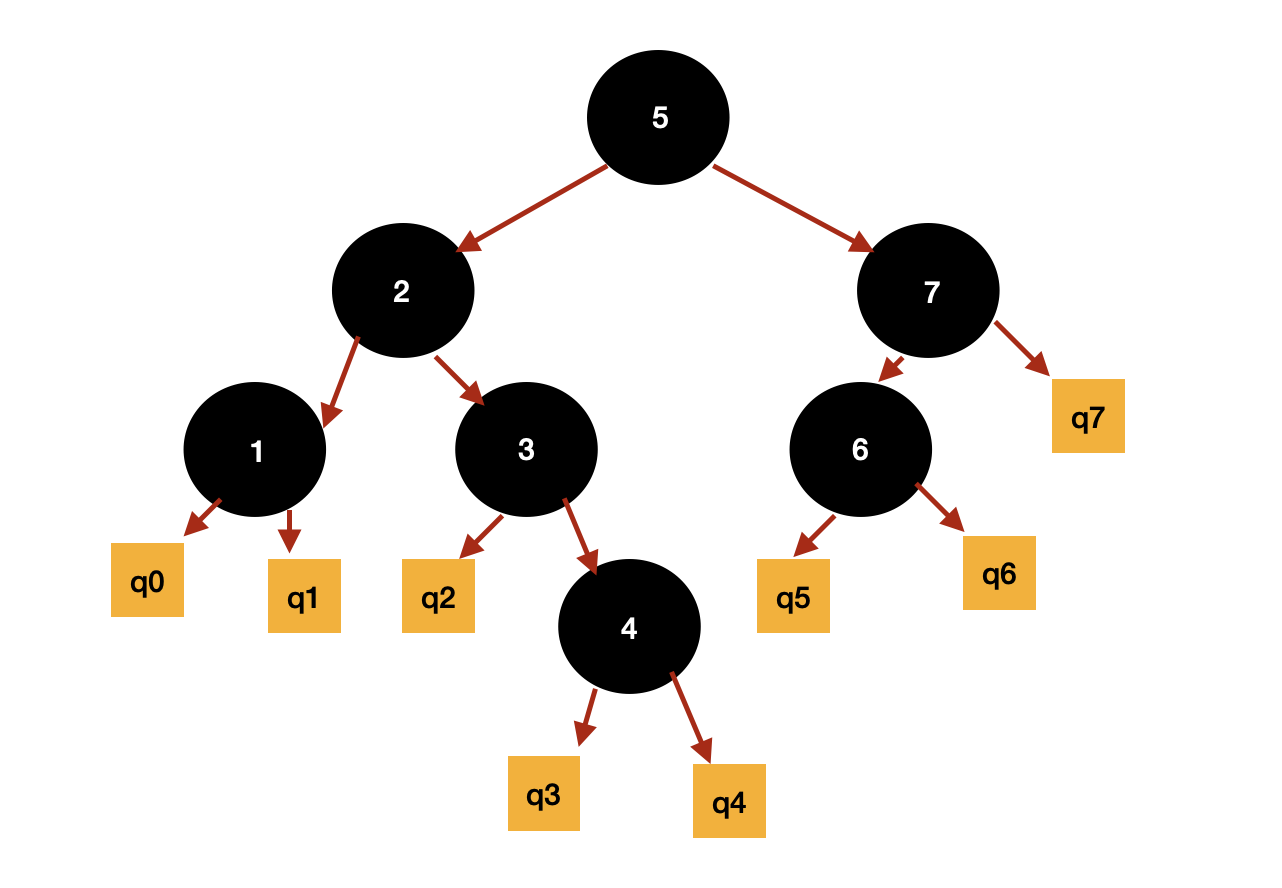
\includegraphics[scale=0.5]{BST Optimal.png}\\
\textit{Optimal BST Visualization}
\end{center}


\pagebreak
\item Problem 5. Reality Check.

        \\
        \textbf{NOTE: }this problem involves writing a short program (in your favorite language). Do not collaborate on the program code, write your own! You may either embed the program in your main PDF, or you may submit it as a separate file. Either way, remember to include a CS "SPCA" comment near the top of your program.\\ \\
        Consider these recurrences, defining M(n) and S(n) for all integers $n \geq 0$:
                
        \begin{equation}
        M(n) = 
        \left\{
            \begin{array}{lr}
                0 & \text{if }  n \leq 1,\\
                M(\lfloor n/2 \rfloor) + M( \lfloor n/2 \rfloor)+n-1 & \text{otherwise}.
            \end{array}
        \right\}
        \end{equation}     
        
        \begin{equation}
        S(n) = 
        \left\{
            \begin{array}{lr}
                M(n) & \text{if }  n < 140,\\
                6*\lfloor n/5 \rfloor) + S( \lfloor n/5 \rfloor)+ S(6 + \lfloor 7n/10 \rfloor) & \text{otherwise}.
            \end{array}
        \right\}
        \end{equation}  
        
        M(n) is the worst-case number of comparisons used by Merge-Sort on n items, and S(n) is (roughly) the worst case number of comparisons used by Select on n items (see Section 9.3). From the book we know that $M(n)=Θ(n*lg n)$ and $S(n)=Θ(n)$, so eventually S(n) is much smaller than M(n).\\ \\
        Write a computer program finding the first n such that $2*S(n) < M(n)$. It should print n, S(n), and M(n). Turn in a copy of your program, and its output.
        \\ \\
        \textit{Remarks: }the first n with $S(n)<M(n)$ is n=154, with $S(n)=974$ and $M(n)=977$. This exercise illustrates that Select does not have much advantage for small inputs (you should probably just sort). The first "6" is the S(n) recurrence is because we can find the median of 5 items using only 6 comparisons (a fun puzzle, but you don't have to solve it). \vspace{2cm}
        
        
        \textbf{Hridansh's Solution on next page}\\
        THIS CODE IS MY OWN WORK, IT WAS WRITTEN WITHOUT CONSULTING \\A TUTOR OR CODE WRITTEN BY OTHER STUDENTS - Hridansh Saraogi


\end{enumerate}
\pagebreak
\textit{A Python program solving Q5, which finds the first n such that $2*S(n) < M(n)$. \\It prints n, S(n), and M(n).}
\lstinputlisting[language=Python]{RealityCheck.py}

\pagebreak
\begin{flushleft}
    Output for code on prev. page (copied from terminal):
\end{flushleft}
\begin{enumerate}
    \item Last element index: 9177855
    \item Last element of S[N]: 101745647; Last element of M[N]: 203491305
\end{enumerate}

\end{document}

